\subsubsection{Detalhamento da Base Mecânica}\label{sec::base_mec}
%TODO Estevão: descrever sistemas de fixação e ancoragem
%TODO Estevão: adicionar subseção de sistema de içamento e entrada dos
% equipamentos 
%TODO Estevão: adicionar subseção do shutter
O estudo da base mecânica investigou primeiramente alguns conceitos baseados nos
graus de liberadade necessários para fornecer à base do robô todos os
posicionamentos necessários para revestimento  da pá, de acordo com os
estudos cinemáticos e dinâmicos. Os graus de liberdade são fornecidos através de
juntas prismáticas e rotacionais, que permitem o movimento do robô desde a
escotilha até o ponto de interesse para o início do processo de revestimento.

A base mecânica deve ser capaz de suportar os esforços dinâmicos do robô, de
forma que não se cause também deformações elásticas e oscilações que possam
comprometer a precisão de posicionamento do efetuador do braço robótico. Deve-se
atentar também ao caráter dinâmico dos esforços, que causam vibrações que devem
ser previstas e evitadas as frequências de ressonância do sistema. Assim, a
fixação da estrutura da base no ambiente deve ser o mais rígida possível,
superdimensionando os elementos de ancoragem e minimizando as folgas nos
acoplamentos.

A entrada dos componentes da base é uma tarefa trabalhosa, devido ao acesso
limitado ao interior da turbina. O diâmetro de $800~mm$ da escotilha limita o
tamanho e geometria dos equipamentos. Além disso, estes componentes devem ser
içados até a escotilha em uma altura de $5~m$ entre o exterior do ambiente
confinado e seu interior. Assim, a modularidade dos elementos que compõe a base
é uma diretriz essencial a esse projeto. A facilidade de transporte, montagem e
desmontagem da base mecânica causará um grande impacto na praticidade e
agilidade de implementação da solução.

A seguir apresenta-se alguns conceitos analisados, em relação aos graus de
liberdade da base mecânica:

$\bullet$~\textbf{Base Prismática-Rotacional-Rotacional (P-R-R):}
  
  Neste conceito estudou-se a possibilidade de utilizar uma base com $3$ graus
  de liberdade: um prismático e dois rotacionais. O prismático seria composto
  por um trilho alinhado e paralelo ao eixo da turbina que transportaria o robô
  até a região próxima a pá. Uma junta rotacional e com eixo vertical orientaria
  a base nesta direção e uma junta perpedincular à primeira faria o
  posicionamento do elo de fixação da base do robô. A figura~\ref{fig::base_prr}
  ilustra este conceito.
    
  \begin{figure}[h!]
   \centering
   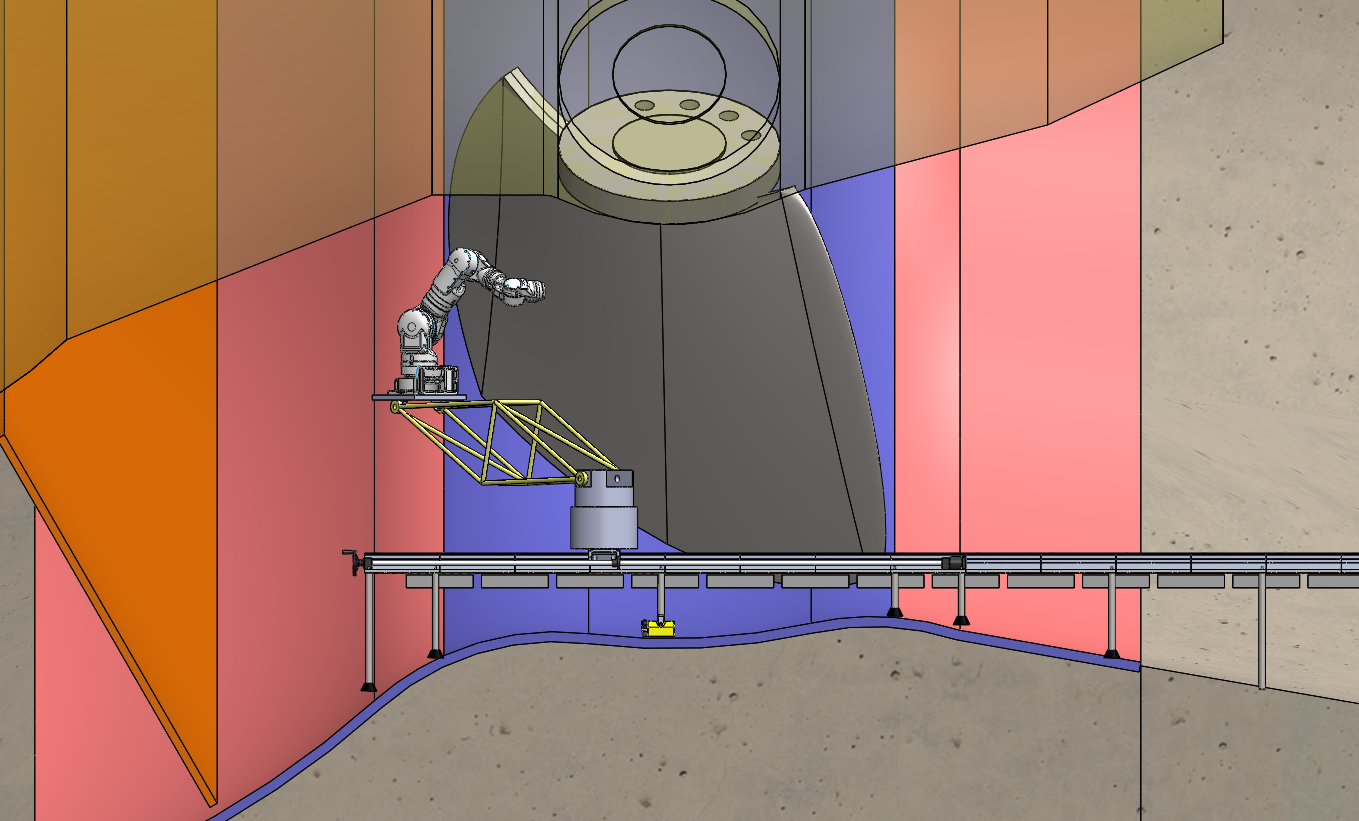
\includegraphics[width=0.8\columnwidth]{figs/bases/base_prr}
   \caption{Base Primático-Rotacional-Rotacional}
   \label{fig::base_prr}
\end{figure}

  Este conceito foi abandonado pela manobrabilidade reduzida da base, devido à
  configuração de juntas, o que levaria a posicionamentos difíceis ou até
  impossíveis de serem alcançados, dependendo do manipulador escolhido.
  
$\bullet$~\textbf{Base Prismática (P):}

  Este conceito consiste de um trilho (junta prismática) para o transporte do
  manipulador desde a escotilha até o ponto de interesse para revestimento na
  face anterior ou posterior da pá. Quando posicionado, remove-se a seção
  do trilho na direção que obstrui a rotação do rotor. Neste conceito,
  adiciona-se um grau de liberdade ao sistema utilizando a própria rotação do
  rotor, posicionando a pá em relação ao robô que é livre no trilho na direção
  do eixo da turbina e fixo nas outras direções. O procedimento para o
  revestimento seria o posicionamento do rotor, o posicionamento do robô no
  trilho, em relação a pá, a ancoragem do robô no ambiente e o revestimento da 
  região possível para aquela posição.
  Repete-se então este procedimento até ter toda a face processada e
  posiciona-se a próxima pá para revestimento, sem necessidade de mover ou
  desmontar a base do robô até todas as faces daquele lado estarem completas.  A
  figura~\ref{fig::base_p} ilustra este conceito.
  
  \begin{figure}[h!]
   \centering
   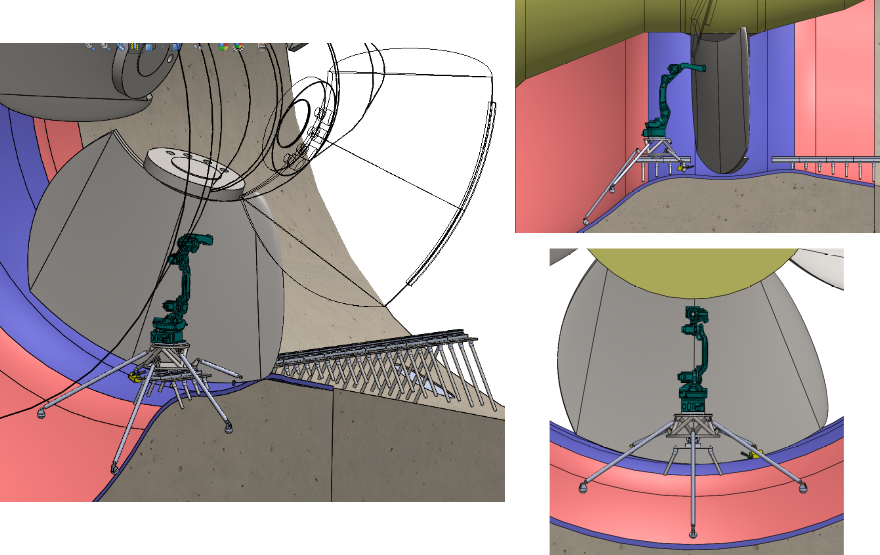
\includegraphics[width=0.8\columnwidth]{figs/bases/base_p}
   \caption{Base Prismática}
   \label{fig::base_p}
\end{figure}

  A análise cinemática demonstrou que seriam necessárias muitas posições do
  rotor para completar uma face da pá. Há inclusive dificuldades operacionais e
  de segurança no procedimento de rotação do rotor que devem ser considerados. O
  rotor só pode ser girado manualmente, não fornecendo precisão no
  posicionamento da pá em relação a base. Por ser uma tarefa manual, deve-se ter
  procedimentos adequados de segurança para preservar tanto o operador quanto os
  equipamentos próximos. Estas preocupações tornam a solução pouco prática sob o
  ponto de vista operacional.

$\bullet$~\textbf{Base Prismática-Rotacional-Prismática (P-R-P):}

  Este conceito consiste de uma base composta por um trilho primário (junta
  prismática $1$), uma plataforma de base pivotada por mancal e rolamentos entre
  o trilho primário e secundário (junta rotacional) e um trilho secundário
  (junta prismática $2$). Montado o trilho primário alinhado ao eixo da turbina
  a base rotacional sobre o trilho primário, fixa-se o robo sobre a base
  rotacional. Esta base permitrá a montagem do trilho secundário apenas quando o
  robô atingir a região de interesse para revestimento. Quando posicionado o
  manipulador, monta-se então o trilho secundário alinhado ao plano paralelo a
  face da pá e ancora-se a base no ambiente. Desta forma, o robô pode-se
  movimentar ao longo de toda a extensão da pá por meio do trilho secundário e
  também se aproximar e se afastar da superfície da pá, por meio do trilho
  primário. A figura~\ref{fig::base_prp} ilustra este conceito.

\begin{figure}[h!]
   \centering
   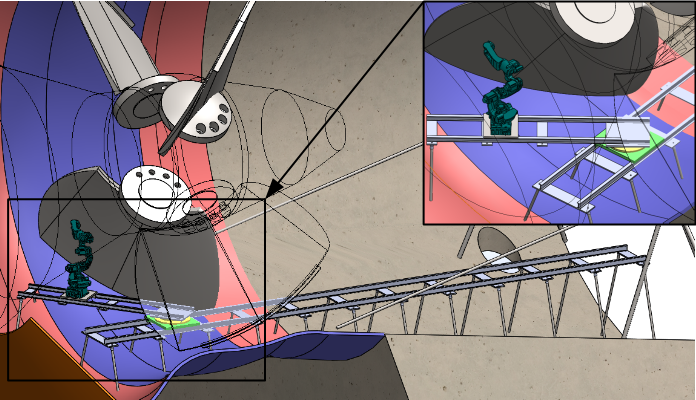
\includegraphics[width=0.9\columnwidth]{figs/bases/base_prp}
   \caption{Base Primática-Rotacional-Prismática}
   \label{fig::base_prp}
\end{figure}

  Desta forma, o rotor deve estar girado em, no mínimo $30^o$ para não haver
  contato com o trilho primário. A análise cinemática será realizada para
  encontrar a melhor configuração de juntas da base que permite ao robô se
  movimentar nos graus de liberdade da base, sem alterar o posicionamento do
  rotor e, assim, cobrir uma face inteira da pá. Para a repetição do processo
  nas outras pás do lado da sucção da turbina, é necessária a desmontagem do
  trilho secundário, o recuo do robô e desmontagem de parte do trilho primário.
  Para as faces do lado de adução, não é necessária a desmontagem parcial do
  trilho primário.
  
  \subsubsection{Sistemas de elevação, fixação e ancoragem}
  A entrada de pessoal através da escotilha é feita por uma escada vertical com
  guarda-corpo com uma altura total de $5~m$. Equipamentos de segurança como
  cinto e talabarte devem ser usados para qualquer um que deseja entrar no
  ambiente confinado da turbina, através da escada e isso impossibilita o
  transporte manual dos equipamentos. Por este motivo, deve ser instalada uma
  estrutura com talha que permita a elevação até o interior da turbina e
  movimentação para a áera de montagem adequada. As figuras~\ref{fig::talha} e
  \ref{fig::talha_trilho} ilustram a estrutura de elevação com talha e carro
  trole. 
  
\begin{figure}[h!]
   \centering
   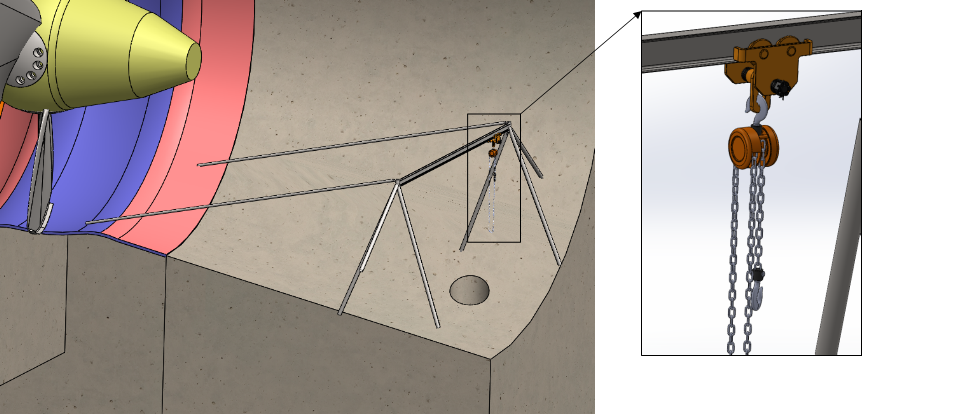
\includegraphics[width=0.8\columnwidth]{figs/bases/talha}
   \caption{Sistema de elevação dos equipamentos}
   \label{fig::talha}
\end{figure}

\begin{figure}[h!]
   \centering
   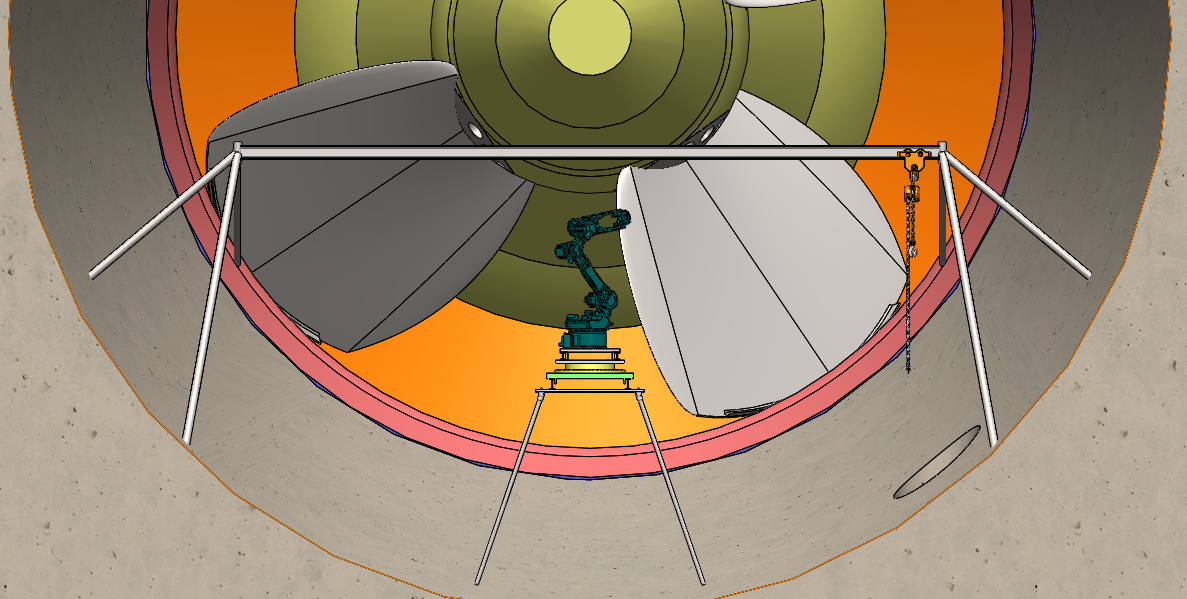
\includegraphics[width=0.8\columnwidth]{figs/bases/talha_trilho}
   \caption{Visão frontal da talha e trilho}
   \label{fig::talha_trilho}
\end{figure}

  Devido aos esforços dinâmicos de operação do robô, a fixação da estutura da
  base mecânica no ambiente deve ser dimensionado com cuidado. Por se
  tratar de uma ambiente de escoamento de fluido sob pressão, não são admitidas
  modificações permanentes de infra-estrutura no interior da turbina, logo,
  qualquer método de fixação utlizado deve ser removível, sem causar nenhum dano
  à qualquer superfície. Em visita técnica realizada em Outrubro de $2015$ foi
  testada a viabilidade de utlização de bases magnéticas para o sistema de
  ancoragem e fixação. Este teste teve o objetivo de verificar a real carga limite de tração
  do imã, considerando o ambiente (geometria), materiais e acabamentos
  superficiais reais a que estará submetido na solução final. O resultado
  detalhado do teste encontra-se no
  %TODO Estevão: incluir ref do Anexo%
  Outra opção para fixação provisória seria a soldagem da estrutura na
  superfície do túnel. Esta opção segue como uma alternativa ainda para regiões
  de difícil fixação da base magnética.
  
  
